\documentclass[12pt,letterpaper,titlepage,en-US]{article}

\usepackage{basicstyle}
\usepackage{report}
\usepackage{knit}
\usepackage{amsmath}
\usepackage{xcolor}
\usepackage{listings}
\usepackage{fancyvrb}
\usepackage{graphicx}
\definecolor{lbcolor}{rgb}{0.969, 0.969, 0.969} 
\setlength\parindent{0pt}
 \lstset{ 
    language=C++, % choose the language of the code
    basicstyle=\fontfamily{pcr}\selectfont\footnotesize\color{black},
    keywordstyle=\color{black}, % style for keywords
    numbers=none, % where to put the line-numbers
    numberstyle=\tiny, % the size of the fonts that are used for the line-numbers     
    backgroundcolor=\color{lbcolor},
    showspaces=false, % show spaces adding particular underscores
    showstringspaces=false, % underline spaces within strings
    showtabs=false, % show tabs within strings adding particular underscores
    frame=single, % adds a frame around the code
    tabsize=2, % sets default tabsize to 2 spaces
    rulesepcolor=\color{gray},
    rulecolor=\color{black},
    captionpos=b, % sets the caption-position to bottom
    breaklines=true, % sets automatic line breaking
    breakatwhitespace=false, 
}


\newcommand{\hmwkTitle}{Mini Project \#5}
\DTMsavetimestamp{DueDate}{2019-04-18T10:00:00-06:00}
\newcommand{\hmwkClass}{CS 6313.001}
\newcommand{\hmwkClassName}{Statistical Methods for Data Science}
\newcommand{\hmwkClassInstructor}{Instructor: Prof. Min Chen}
\newcommand{\hmwkAuthorName}{Shyam Patharla}
\newcommand{\hmwkAuthorNetID}{sxp178231}

\newcommand{\hmwkAuthorOneName}{Lizhong Zhang (lxz160730) : P1(ae), P2(bcde)}
\newcommand{\hmwkAuthorTwoName}{Hanlin He (hxh160630) : P1(bcd), P2(af)}



%
% Title Page
%

\title{
    \vspace{1in}
    \textmd{\textbf{\hmwkClassName \\\hmwkClass:\ \hmwkTitle }}\\
     \normalsize\vspace{0.1in}\small{Due\ on\ \DTMusedate{DueDate}\ at \DTMusetime{DueDate} }\\
    \vspace{0.1in}\large{\textit{\hmwkClassInstructor}}\\
    \vspace{0.5in}
\includegraphics[height=2.4em]{UTD_logo_BW}\\
    \vspace{2in}
}

\author{\textbf{\hmwkAuthorName\ \footnotesize{(\hmwkAuthorNetID)}} \\ }
\date{}
\makeindex

\begin{document}
\maketitle

\pagenumbering{Roman}

\tableofcontents

\pagebreak
\pagenumbering{arabic}


\section{Answers}

\subsection{}

\subsubsection{Do males and females differ in body temperature?}
Let us first formulate the hypotheses:\\
Null Hypothesis, $H_{0}: \mu_{x}=\mu_{y}$ (male and female body temperatures are same)\\
\indent Alternate Hypothesis, $H_{1}: \mu_{x} \neq \mu_{y}$ (male and female body temperatures are different)
\\

 Let us make a boxplot first.


\includegraphics[scale=0.6]{body-temp.jpeg}\\


Inferences:
\begin{enumerate}
\item We see that the two distributions do \textbf{differ} in some respects. 
\item The female distribution has a higher \textbf{median} body temperature.
\item The female distribution has some \textbf{outliers} on both ends.
\item The male distribution has a slightly \textbf{wider} interquartile range.
\end{enumerate}


We compute a 95\% CI for two cases:
\begin{enumerate}
\item Assuming equal variances: \textbf{[-0.53963938 -0.03882216]}
\item Assuming unequal variances: \textbf{[-0.53964856 -0.03881298]}

\end{enumerate}
Both approaches yield \textbf{similar} confidence intervals for the difference in means. These confidence intervals suggest that the difference in means is \textbf{significant}, supporting \textbf{$H_{1}$}.\\

We finally confirm our conclusions with a \textbf{T-test}. Suppose:\\
\textbf{x.mean}= mean body temperature for males \\
\textbf{x.sd}= standard deviation for body temperature for males\\
\textbf{n}=number of males\\
\textbf{y.mean}= mean body temperature for females \\
\textbf{y.sd}= standard deviation for body temperature for females\\
\textbf{m}=number of females
\begin{knitrout}
\definecolor{shadecolor}{rgb}{0.969, 0.969, 0.969}\color{fgcolor}
\begin{kframe}
\begin{verbatim}
> t_obs <- (x.mean-y.mean) / sqrt((x.sd^2/n) + (y.sd^2/m))
> p_value <- 2*(1 - pt(abs(t_obs),df))
> p_value
# [1] 0.02393826
\end{verbatim}
\end{kframe}
\end{knitrout}

Assuming a 5\% level of significance,\\
\begin{equation}
p-value = 0.02393826 < 0.05
\end{equation}
Hence, we \textbf{reject $H_{0}$}. Hence males and females differ in body temperature.

\subsubsection{Do males and females differ in heart rate?}
Let us first formulate the hypotheses:\\
Null Hypothesis, $H_{0}: \mu_{x}=\mu_{y}$ (male and female heart rates are same)\\
\indent Alternate Hypothesis, $H_{1}: \mu_{x} \neq \mu_{y}$ (male and female heart rates are different)
\\

 Let us make a boxplot first.


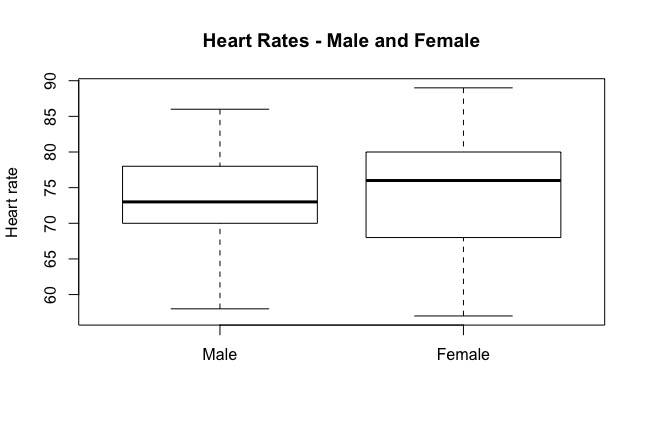
\includegraphics[scale=0.6]{hrate.jpeg}\\


Inferences:
\begin{enumerate}
\item We see that the two distributions do \textbf{differ} in some respects. 
\item The female distribution has a higher \textbf{median} heart rate.
\item The female distribution has a slightly \textbf{wider} interquartile range.
\end{enumerate}


We compute a 95\% CI for two cases:
\begin{enumerate}
\item Assuming equal variances: \textbf{[-3.241461, 1.672230]}
\item Assuming unequal variances: \textbf{[ -3.243732,  1.674501]}

\end{enumerate}
Both approaches yield \textbf{similar} confidence intervals for the difference in means. These confidence intervals indicate that the differences in means \textbf{could} be zero, but we don't have enough information to make our decision. \\

Hence, we proceed with a \textbf{T-test}. Suppose:\\
\textbf{x.mean}= mean heart rate for males \\
\textbf{x.sd}= standard deviation for heart rate for males\\
\textbf{n}=number of males\\
\textbf{y.mean}= mean heart rate for females \\
\textbf{y.sd}= standard deviation for heart rate for females\\
\textbf{m}=number of females
\begin{knitrout}
\definecolor{shadecolor}{rgb}{0.969, 0.969, 0.969}\color{fgcolor}
\begin{kframe}
\begin{verbatim}
> t_obs <- (x.mean-y.mean) / sqrt((x.sd^2/n) + (y.sd^2/m))
> p_value <- 2*(1 - pt(abs(t_obs),df))
> p_value
# [1] 0.5286842
\end{verbatim}
\end{kframe}
\end{knitrout}

Assuming a 5\% level of significance,\\
\begin{equation}
p-value = 0.5286842 > 0.05
\end{equation}
Hence, we \textbf{accept $H_{0}$}. Hence males and females do not differ in heart rate.



\subsubsection{Is there a linear relationship between body temperature and heart rate? Does the relationship depend on temperature?}
Let us first make a scatterplot of body temperature against heart rate for all genders.

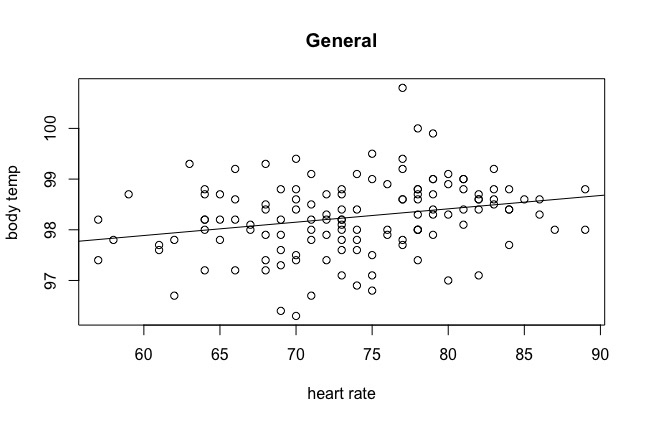
\includegraphics[scale=0.6]{linear.jpeg}\\

Let us now make scatterplots of body temperature against heart rate for males and females.
\includegraphics[scale=0.6]{male-linear.jpeg}\\
\includegraphics[scale=0.6]{female-linear.jpeg}\\

\begin{enumerate}
\item The correlation coefficient is $\rho=0.2536564$ for the whole population. The data does not fit the line well.

\item The correlation coefficient is $\rho=0.1955894$ for the male population. The data does not fit the line well.

\item The correlation coefficient is $\rho=0.2869312$ for the female population, higher than the $\rho$ for the male and whole population. The data does fit the line well compared to the male distribution.

\item We can conclude that:
\begin{enumerate}
\item there is \textbf{no} linear relationship between heart rate and body temperature for the \textbf{whole} population.
\item  there is \textbf{no} linear relationship between heart rate and body temperature for \textbf{males}.
\item there \textbf{might} be a linear relationship between heart rate and body temperature for \textbf{females} but the strength of the linear relationship is not very high.
\end{enumerate} 
\end{enumerate}


\subsection{}
\subsubsection{For a given setting of (n,lambda), compute Monte Carlo estimates for coverage probabilities of the 2 individuals}
Let n=30, $\lambda$=0.1, nsim=5000. We get:
\begin{knitrout}
\definecolor{shadecolor}{rgb}{0.969, 0.969, 0.969}\color{fgcolor}
\begin{kframe}
\begin{verbatim}
> cover.probs(30,0.1,5000)
# [1]  0.9136 0.9360
\end{verbatim}
\end{kframe}
\end{knitrout}
The coverage probability for both the large-sample and bootstrap intervals is slightly \textbf{less} than our confidence level of 95\%.



\subsubsection{Repeat (a) for remaining combinations of (n,lambda) and present a summary of the results}
\begin{table}[H]
\centering
\begin{tabular}{|c|c|c|c|c|}
\hline
& $\lambda=0.01 $  &$\lambda=0.1 $   &$\lambda=1$    &$\lambda=10$ \\\hline
n=5	&0.8098 	 &0.8204	&  0.7974   & 0.8124\\\hline
n=10	&	0.8652 	&0.8696	&0.8732	&0.8748\\\hline
n=30	&0.9152 	&  0.9136 &0.9166	 &0.915 	\\\hline
n=100	& 0.9412 	&0.9368	 &0.9434	&0.9422\\\hline
\end{tabular}
\caption{Coverage probabilities for large-sample interval }\label{1}
\end{table}



\begin{table}[H]
\centering
\begin{tabular}{|c|c|c|c|c|}
\hline
& $\lambda=0.01 $  &$\lambda=0.1 $   &$\lambda=1$    &$\lambda=10$ \\\hline
n=5	&0.8968 	 & 0.8970	&  0.8984  &0.9006\\\hline
n=10	&0.9222 &0.9152 	&0.920	&0.9156\\\hline
n=30	&0.9366 	&0.9360	 &0.9366 	&0.9434\\\hline
n=100	&0.9442 	&0.9420	 &0.9476	&0.9430\\\hline
\end{tabular}
\caption{Coverage probabilities for bootstrap interval}\label{1}
\end{table}



\subsubsection{Interpret the results}
Inferences for both intervals:
\begin{enumerate}
\item For a given value of n, the coverage probability \textbf{does not change} much with respect to $\lambda$.
\item For a given value of $\lambda$, the coverage probability \textbf{increases} with increasing n. 
\item The coverage probabilities for n=100 are \textbf{closest} to our confidence level of 95\% irrespective of $\lambda$.
\end{enumerate}


Sub-questions:
\begin{enumerate}
\item For the large sample interval, how large does n have to be for the interval to be accurate?\\
The large sample interval gives coverage probabilities close to our confidence level of 95\% for n$=$100.


\item For the bootstrap interval, how large does n have to be for the interval to be accurate?\\
The bootstrap interval gives coverage probabilities close to 0.95  for for n$=$100.

\item Do these answers depend on $\lambda$?\\
No, the answers to the above questions \textbf{do not} depend on $\lambda$.

\item Can we say that one method is more accurate than the other? Which interval would you recommend?\\
The bootstrap interval appears to be working \textbf{better} for smaller n. But for large n, both are equally good irrespective of $\lambda$. \\
I would recommend the \textbf{bootstrap} interval.

\end{enumerate}



\subsubsection{Do the answers to (c) depend on the specific values of lambda that were fixed in advance?}
No, the conclusions in (c) \textbf{do not} depend on $\lambda$.











\section{R Code}
\lstinputlisting{/users/psprao/downloads/stats/mini5/Q1A.R}
\lstinputlisting{/users/psprao/downloads/stats/mini5/Q1B.R}
\lstinputlisting{/users/psprao/downloads/stats/mini5/Q1C.R}
\lstinputlisting{/users/psprao/downloads/stats/mini5/Q2.R}


\end{document}
